% !TeX spellcheck = en_GB
\documentclass[a4paper,english]{report}
\usepackage[utf8]{inputenc}
\usepackage{babel,duomasterforside}
\usepackage{amsmath}
\usepackage{amsfonts}
\usepackage{amssymb}
\usepackage{graphicx}
\usepackage{listings}
\usepackage{gensymb}
\usepackage{color}
\usepackage{natbib}
\usepackage{csquotes}

\setcitestyle{square}
\title{The power of a Multiagent Orchestra}
\subtitle{A trying time for all}
\author{Halvor Sogn Haug}
\begin{document}
	\duoforside[dept={Institute of informatics},
	program={Informatics: Robotics and Intelligent Systems},
	long]
	\begin{abstract}
		I'm so cool yo
	\end{abstract}
	\tableofcontents
	
	\chapter{Introduction}
	Music has long been one of the central ways for humans to express themselves creatively. From all the way back in prehistoric times, until now in the modern world, music has been a form of creative expression. With the advent of the computer age, the ways of expressing yourself have only expanded more. With synths, music software, and audio processing techniques, there are more ways to express yourself musically than ever. But while there are many possibilities, most are either unknown or not well documented, which makes it harder for people to take advantage of these possibilities. 
	\\
	To help shed light on this possibility space, this thesis will investigate how people can interact with a system designed from 
	\section{Thesis goals}
	The goals of this thesis are to:
	\begin{itemize}
		\item Develop a musical system based on Swarm Intelligence to allow for a new type of musical expression.
		\item Conduct a user study to investigate how people interact with the developed system.
	\end{itemize}
	These are the corresponding research questions:
	\begin{itemize}
		\item Can Swarm Intelligence allow for a new kind of musical experience?
		\item How do people interact with a swarm based music system?
		\begin{itemize}
			\item How does the level of control affect the user's experience?
		\end{itemize}
	\end{itemize}
	\section{Contributions}
	\chapter{Background}
	\section{Introduction}
	The ubiquity and popularity of music as a creative task makes it a very attractive task for artificial intelligence (AI) research, not just for the creation of music itself, but also for research into creative activities in general. This field, concerned with using technology and algorithms to work with music, is called Musical Metacreation. Musical metacreation is defined as ``\textit{a subfield of computational creativity that adresses music related tasks}" \cite{pasquier2017introduction}. This does not only cover the creation of new music itself, but also real-time improvisation and accompaniment.\\
	Multiagent systems are systems that instead of using a single agent to make decisions, uses multiple agents making individual decisions instead, that can create a greater whole  together through emergence. Emergence is a term describing properties a system can have, that appears despite none of the individuals in the system having them.
	
	\section{Musical metacreation}
	The approaches to the process of musical metacreation are many and varied, depending on the goal. For example, you can hardcode in rules from music theory, or use machine learning to find the rules by itself. There's also a big difference between if the system itself is autonomous, interactive, or something in between. The system can also be offline, where the output isn't concerned with any real world interaction, or it can be in real-time, where the timing in relation to the real world matters.
	
	\subsection{Interactive vs. Autonomous}
	The difference between an interactive and an autonomous system, is that the interactive system allows the user to influence the behaviour, meanwhile an autonomous system will need no input after it has started.\\
	The benefit of using an interactive system is that it allows a human to control and influence how the output will sound. The system is therefore almost more like an instrument, in how the user uses it to ``play". This also means that the system might not need a strict evaluation of its own output, as the user is able to influence it, and therefore able to act as an evaluator to the output. The main drawback of the direct systems is that you need a user to actively interact with the system for it to work well, and it could be argued that the system is not producing pleasant sounds on its own, but rather by the user's evaluation. This can be done in various ways, for example, you can have the user directly curating the output \cite{studley2019exploring},  is responsible for organizing the system \cite{bennett2018neurythmic}, or the human user is directly giving inputs into the system that it adjusts and adapts to \cite{blackwell2003swarm}.\\
	When the user is curating they the output, the system is creating many different melodic ideas, in which the user is curating and removing those that they find displeasing. In Studley et al.'s paper, the user is playing a game.  This encourages the user to remove the musical ideas they don't like, while also constantly having new musical ideas show up, creating a dynamic experience. This approach is also different from other interactive approaches, where the human user gives some input that the system react to, here it's the system that creates musical ideas, and it's up to the user to react and respond to it.\\
	For systems where the user is organizing it, as in Bennet's paper on Neurhythmic, where central pattern generators (CPGs), who are oscillators that can influence each other, the user is responsible for creating and placing these generators. This is able to create novel musical ideas.\\
	Lastly, there are the systems where the user gives input directly. They are generally reactive systems, and will not produce musical ideas on their own. Rather, they work on embellishing on the ideas given as input, and are therefore often used for accompaniment.\\
	On the other hand there are autonomous systems, who do not require any input from humans at all, and can run on their own. As these systems are working on their own, they need some kind of evaluation to determine how good the created music is, however they are also able work offline, which means that they can look at the whole of the musical output to create a structure, as opposed to real time systems, which are closer to improvisation.
	
	\subsection{Harcoded rules vs. Machine Learning}
	The main benefit of hardcoding the rules, is that you can ensure it follows some kind of musical framework, which in turn will increase the quality of output produced. The drawback on the other hand is that it can often get restricted by the rules, which can limit the variety of the musical output.\\
	When you hardcode musical rules, there are multiple approaches you can take, that also depends on if the system is interactive or autonomous. For an autonomous system, some degree of stochasticity is needed to not have the system have the exact same output over and over. And example of this is Farbood et. al's paper on synthesizing music for Palestrina-style counterpoint \cite{farbood2001analysis}. In the paper, they set up tables with probability transitions between notes in terms of the intervals, and used that combined with Markov Chains to predict the next note that should be played. It is also worth mentioning that while they hardcoded the musical theory rules, they still took advantage of machine learning techniques to combine it together for the final output.\\
	Using counterpoint was also built on by Plutt et. al, in their paper on LazyVoice \cite{plutt2021lazyvoice}. LazyVoice is a multi-agent system focused on creating pleasant harmonies. This is done by using voice leading, specifically that notes should move to the closest possible note that fits into the chord selected. Each individual agent is represented as being a voice line, and has parameters for how long each note will be, how deep into the chord it will look to find an appropriate note (so it can play 7th and 9th chords), and is also able to be influenced into moving either away from or towards other notes.\\
	The opposite to hardcoding rules would be musical systems that takes advantage of machine learning in some way. This can either be done by having the system learn the rules from a corpus, or it can try to learn the rules through some evaluation function.\\
	Learning from a corpus, the main goal is to in some way imitate the music the corpus consists of, and use that as a basis for learning rules. For example, in Tatar et. al's paper on using self-organizing maps \cite{tatar2017masom}, the training set consists of music of one style that should be imitated. Self-organizing maps are a method for reducing the dimensionality of a set of data, and this is used to classify different "sections", or repeating ideas in the corpus. This allows the entire musical piece to be sliced into smaller parts that are each marked as a category, and then they can use that string of categories to train a Markov Chain. However, it is important to note here that the way the self-organizing maps are able to reduce the dimensions, is by looking at the features extracted from the audio. These features, which are based on a calculation of the valence and arousal of any particular sound, are implemented by hardcoding in a formula for them. This is a general principle for most systems that take advantage of machine learning in some way, that some part of it will have to be hardcoded. This is because the use of heuristics are a natural part of Artificial Intelligence, as the space the algorithm can work in tends to be too big otherwise.\\
	The self-organizing maps from MASOM was also used in StyleRank, a system for classifying music based on style in some way, whether it be genre or composer \cite{ens2020quantifying}. As it is focused on learning the rules, to be able to classify the music, it is mainly using Machine Learning. However, as with MASOM, the way the music is able to be classified is by extracting features, which requires some hardcoding.\\
	For systems where the user is responsible for organizing the system, such as Neurhythmic mentioned earlier, at least part of the hardcoded rules or machine learning is substituted by the human participant. In Neurhythmic for example, the user is responsible for structuring the CPGs and connecting them together, which is then used to generate rhythm \cite{bennett2018neurythmic}. As the rhythm generation is done by playing according to the CPGs, whose main behaviour is largely dependent on their connections and whether they resonate with them, 
	\iffalse
	\subsection{Neurythmic}
	Bennet's paper about Neurythmic shows an interesting example of using biological models for musical metacreation. By using central pattern generators (CPG), which are usually used to simulate walking patterns, he is able to generate rhythmic patterns in an environment that influences each other. This is done by having the different CPGs be  nodes in an environment, who can be connected and through that influence other CPGs.\\
	This is able to create novel and interesting rhythms, however it is dependent on a user placing the rhythm nodes themselves, and said placement can also influence the quality of the musical output itself. In addition, the system is mainly focused on creating rhythm, and melody would have to be handled separately.
	
	\subsection{MASOM}
	Masom, presented in a paper by Tatar et al. \cite{tatar2017masom}, is a musical agent who has been taught music, through the use of self-organizing maps. By using self-organizing maps, the agent is able to learn a particular style of music, specifically it's able to categorize the types of musical movements into general categories. Afterwards, it uses a Variable Markov Model to predict the way the categories should be ordered when generating music.\\
	They also performed experiments by having multiple agents perform together, and also with a human participant, where the entire audio environment is evaluated by the Markov Model to predict what category should be played next. When it chooses a segment to play, it selects a random sample from that category to play. This means that the played sample might not fit perfectly to the music, depending on how the data is clustered.\\
	Another thing to consider is that while the self-organizing maps make sure the samples played will "fit in" with the musical landscapes, it also limits the output to the range of samples given to it during training. This means that the musical output will always be limited to the training data, and it can't try anything not done before.
	
	\subsection{StyleRank}
	Ens et al presents StyleRank, a method of classifying MIDI-files to see how well a MIDI file fits to an arbitrary musical style \cite{ens2020quantifying}. It does this by taking the chords, and comparing the pitches relative to the chord that is being played, and extracting various features from the midi file. Then, learns to classify the midi by using random forests.\\
	The system has shown itself able to predict both which works were written by which artists, at a level comparable to humans. An important observation is that using the Euclidean distance gives poor performance. The main drawback to this approach is that it requires an existing corpus to compare to.
	
	\subsection{Competitive Musical Creativity}
	An interesting experiment was done by combining computer games with musical metacreation, by Studley et al. \cite{studley2019exploring} What they did, was create two games, that would produce some kind of musical output when the user played it. The first game created was based on cells, specifically mitosis and evolution. Each cell in the game creates a musical event, and the user controls the musical output by destroying cells until the desired output is reached. In addition, over time, the cells can split, and create new musical events, which is determined by a stochastic process. Therefore, the user has to stay vigilant, and manage the cells so that the output is close to what the user desires.\\
	The other game created, is a simple game where the player has to run from a pursuer. The musical output is determined by the distance between the player and the pursuer, as well as which environment the user is currently in. This creates a dynamic process, where the player has to stay engaged to not lose the game.\\
	While these games are interesting, the main drawback is that they still require a human component to perform. As the user is the one who curates the musical output by their decisions, the judgement of if the musical output is "good" is left to the person interacting with the games. While this is certainly useful for getting pleasant-sounding musical output, it also means that the system is dependent on a user directly interacting with it.
	\fi
	
	\section{Multi-agent systems}
	There are generally two types of multiagent system: \\
	The first one is swarm intelligence, which uses simple agents and takes a lot of inspiration from nature. These agents follow simple rules often based on the 'senses' of the agent. \\
	The second one is based on economics and sociology, and uses more complex agents applying game theory to take the action that benefits themselves the most. 
	
	\subsection{Swarm intelligence}
	Swarm Intelligence is characterized by six properties of the agents \cite{bonabeau1999swarm}. Those six are:
	\begin{samepage}\begin{enumerate}
		\item Autonomy
		\item Distributedness
		\item Simple agents
		\item Emergence
		\item Stigmergy
		\item Self-organization
	\end{enumerate}\end{samepage}
	Autonomy means that each agent is able to move about and operate on its own, independent from any other agents. This is a trait common to all agents in a multi-agent system, also agents that apply game theory.\\
	Distributedness means that there is no central control sending signals and directing the agents. Rather, the agents are taking all decisions independently, and on their own. This means that the system only requires the simulation of the agents and environment, and not an organizer that keeps track of every agent.\\
	Simple agents means that the agents do not have complex thoughts, but instead make decisions based on a set of rules, usually by using some kind of sensor input to determine what action to take. For example, in the ant colony optimization algorithm the agents will choose which path to take randomly, but will be more likely to choose paths with a heavy pheromone trail.\\
	Emergence means that the simple interactions the agents have with each other, when seen as the whole, will create some kind of greater effect. This emergent effect could be said to be the goal of the swarm system itself.\\
	Stigmergy is how the agents communicate with each other, which is not directly, but rather indirectly by changing the environment. This can be by laying out pheromone trails, making sounds, or by stopping and becoming an obstacle in the environment themselves. This also means there's no need to implement communication protocols between agents, since they all instead simply interact with the environment.\\
	Self-organization means that the swarm of agents organizes itself on its own. This specifically matters in situations where there are different tasks that needs to be done, or where more than one agent is needed to complete a task. The main benefit of this, is that it makes the swarm flexible and robust, so even if some agents either go offline or crash, the rest of the swarm can still operate, or that there are no essential individual agents.\\
	Lastly, while this isn't a formal requirement, it is usual for swarm intelligence systems to consist of a large number of agents, usually 100 or more. This allows the system to be more stable in regards to self-organization, as the loss of one agent is more critical the fewer total agents the are. As the agents will always follow simple rules, it's also easier to scale up the number of agents, as each agent needs less processing power.
	
	\subsubsection{Interactive Swarm Orchestra}
	At the Zurich University of the arts, Bisig et al. has been working on applying swarms to an interactive orchestra, that they've been conducting quite a few experiments with \cite{bisig2008interactive}. The system consists of different modules, but the ones of most interest here are the synthesis and flock modules. The synthesis module is focused on converting various inputs into an audio output. As it is a general framework, there is no specific method introduced for converting to audio. The flock module is also a general framework for doing swarm simulations, whose parameters in the space will be passed along to the synthesis as either input or control parameters.\\
	The system has later been expanded to include experiments where the whole system has been turned into an instrument, with specific tools for a human participant to influence the swarm and therefore its output \cite{bisig2012tools}. Out of this has also come research into what parameters are good to use when using swarms for musical metacreation.There have also been forays into having the system interact with external devices that work as instruments, which can interact with and influence the swarm. Suggested has been both using the position of the swarm(s) to determine the amplitude and frequency of oscillators, or to combine it with granular synthesis. It is also suggested that you could use the distance between the swarm agents as parameters.\\
	The main interest with this system is it being one of the first general swarm music systems, meaning that it is not bound to any particular implementation or algorithm, but rather is able to support any of them if implemented. In this way, this is more of a framework than one particular implementation, but it does also suggest a structure for similar projects, in that the swarm implementation and synthesiser could be kept seperate to avoid interaction. There may be some benefits to having them interact though, such as letting audio events influence the actions of the swarm directly.
	
	\subsubsection{Boids}
	One of the most common algorithms to use for creative swarms is the boids algorithm, which simulates the flocking behaviour of birds. The algorithm was presented by Reynolds in 1987 \cite{reynolds1987flocks}, and it consists of individual agents who follow three simple rules:
	\begin{samepage}\begin{enumerate}
		\item The agents should adjust their path so they don't collide with nearby agents.
		\item The agents should attempt to match the velocity of the agents around them.
		\item The agents should try to stay close to the agents around them.
	\end{enumerate}\end{samepage}
	These three rules will ensure that the agents stay together with out colliding, and that they move in the same directions. The rules can also be expanded to include obstacle avoidance, which lets the agents move around in a simulated environment. \\
	The boids model fits all the requirements for a swarm model, as the agents are autonomous and make decisions on their own, they only follow a set of simple rules, the flocking behaviour emerges from the agents following those rules, they change the environment for communication by themselves moving around, and the swarm is very flexible to the number of agents present, even if some were to be defective.\\
	The reason the boids algorithm is used so much, is that unlike many other swarm algorithms, it is very open-ended. Where most swarm algorithms have an optimization goal they want to achieve, and that the agents will work towards solving, the boids do not have that, and the main behaviour is rather moving around in a coordinated fashion. This is particularly good for musical endeavours, as coordinated movements is something that often show up in music.\\
	One of the first implementations of boids for musical purposes was done by Unemi et. al \cite{unemi2005music}. In their paper, the boids agents moved around in a 3D space, where the coordinates are mapped to represent pan, pitch, and velocity. In addition, the swarm was able to be interacted it by filming human participants, who the swarm then corresponded to in how they moved. The various parameters that swarm algorithms could use to convert into musical ideas was also expanded on by Bisig et. al in 2008 \cite{bisig2008swarm}. The most basic is similar to what they did with boids, where the coordinates are directly translated into pan, pitch and velocity for the notes. It's also possible to take it a step further and have the coordinates correspond to parameters for oscillators, which will then generate music when added together. Alternatively, it is possible to use granular synthesis, a method where the audio is split up into small samples that are then later modified by adding them together or modifying their parameters such as the speed they're played at, their amplitude, their phase, and so on. You can then have those parameters decided by the agents' position, velocity, and distance to other neighbours, to create audio output.\\
	Using a camera to have the user interact has also been done in the SwarmArt project, where boid swarms could be interacted with by human participants over film. \cite{boyd2004swarmart}. Here, the swarm is given the coordinates of objects that move in front of the camera, and use those to determine where to go. The main benefit of using a camera for human participation is that it allows for an easy and intuitive way for anyone to be able to interact with the swarm.
	
	\subsubsection{Multi-swarms}
	Multi-swarms are swarm systems that take advantage of having multiple separate swarms existing in the space \cite{blackwell2004multi}. The main benefits to this approach is that they can be better for solving problems where the search landscape is dynamic, and can change over time. Blackwell have already used this approach to create a system that produces musical output, both by its own and in conjunction with human participants \cite{blackwell2003swarm}. It works by using multiple particle swarm optimization swarms, who consist of particles being attracted toward the best spot they've found themselves as well as the best spot the swarm has found, and these swarm then exist simultaneously in the same environment. The 3d environment space represents the loudness, pulse, and pitch of the tone. It then captures both internal and external audio events, and uses them as basis for the target points of the swarm. How the targets are decided is determined by scripts, who process the audio events, mostly to prevent convergence and to make sure the swarms are spread out.
	\iffalse
	\subsubsection{SwarmArt}
	SwarmArt is an art installation that lets human participants to interact with a swarm. This is done by using video cameras to film the location of the human participants, and therefore use them as inputs to the swarm system. This way, the participants are able to influence the swarm with their movements, and seeing it change.
	\fi
	\subsection{Game Theory}
	Game theory agents differ from swarm intelligence agents in that instead of just following rules, they try to observe the environment around them, and deliberately choose the option that will benefit themselves the most \cite{wooldridge2009introduction}. They are also able to establish communication protocols for directly talking with each other, so they can try and come to decisions that are mutually beneficial. As the agents have to evaluate their environment, and then predict the most beneficial actions for themselves based on what other agents will choose, game theory agents require significantly more processing power than swarm agents. Due to this, the number of game theory agents you can have running in simulation will be fewer, and they will also be more expensive to manufacture for real world operations.\\
	Unlike swarm intelligence systems, game theory systems usually require more processing power from each agent, as they're expected to evaluate and predict other agents' actions as well. This means that the number of agents tends to be smaller than for a swarm system, and as the rules are more explicitly coded into the agents as well, there is less of an ``emergence", regarding the behaviour of the system.\\
	The common aspect to all of the following examples using game theory agents is that unlike the swarm systems, the rules are very finely tuned towards the task they're supposed to solve. In addition, the number of agents are generally quite few, but they can allow for human participants to take part as one of the agents, instead of influencing the entire system as is common in the swarm projects.	
	
	\subsubsection{Agents talking with each other}
	There are multiple ways to implement game theory agents, and one of them, is implementing agents which directly talk with each other out loud in real time and try to anticipate what to do based on the audio input they get. Examples of this type of agent can be seen in Boersen et. al's paper on Chatterbox, an art installation for the purpose of simulating multicultural communication \cite{boersen2020chatterbox}. This is done by having Chatterbox agents, who are able to generate gibberish vocal streams, that has no meaning. This is done by using self-organizing maps to categorize human speech, specifically the MASOM system mentioned earlier. Afterwards, the agents are given instructions on how to interact with each other, with different layers. Layer 1 is for example to start speaking if there's silence, and to stop after it has ``finished speaking" so to say. Additional layers of rules, including trying to predict when other agents will finish speaking so they can start speaking themselves, leads to a dynamic behavior where the agents are in constant conversation with each other. \\
	This installation is also similar to Rokeby's n-Cha(n)t installation, in that it features various agents communicating with each other, that can also listen to the human speakers who are there \cite{rokeby2001nchant}. However, while in Chatterbox the agents try to hold a conversation by speaking in turn and not interrupting each other, in n-Cha(n)t the agents will rather synchronize if left unattended, and start chanting. If they recieve outside stimuli from a human, they will try to process what they hear, and add on to that. \\
	An interesting part of these types of set-up is how they work through real space, and also incorporate human participants, which allows for the system to be both automatic and interactive. This could also be done in some kind of virtual environment where the user is allowed to walk around, to maintain the idea of space and location mattering, which can be quite useful for auditory tasks. Another interesting factor is how the systems all listen to each other and try to act according to what they hear, essentially having to anticipate what the other agents will do, which is very useful for musical tasks, as you need to anticipate what the other agents will play so you can harmonize with them. This is especially useful when it comes to improvisational tasks, or where the system works real-time.
	
	\subsubsection{Passing it around}
	Another technique that can be used for implementing game theory agents, is the mechanism of passing either responsibility or the output around between the agents, and in the period where an agent have responsibility, they have full control. This can be done both in real-time or offline, depending on the system.\\
	An example of this comes up in Chandra et. al's paper on SoloJam, which uses auctioning theory to distribute the time a participant can play a solo \cite{chandra2012market}. This is done by having the agent/node that is currently performing a solo auction off the right to continue the solo, using a sealed-bid, second price auction, also known as a Vickrey auction. Each node bids with its own rhythmic pattern, and the amount bid corresponds to the evaluation of the rhythmic pattern. This will ensure that it's always the best rhythmic pattern that will have the solo. This system works in real-time, and the responsibility for the solo is passed around between the participants as they play.\\
	Another example of this can be seen in Kirke et al.'s paper on multiagent poetry.\cite{kirke2013emotional} By giving each of the agents a "mood", based on valence and arousal, they had the agents select appropriate words corresponding to their mood for their poems, then it was passed around to another agent. After reading the poem that they've received, their mood is affected by the contents of the poem, and then they added text to the poetry based on their new mood. This process continues until the program is stopped. The result is a set of poems that are filled with repetition, but has a somewhat recursive structure  to itself. While the poems in text form appear quite nonsensical, this might work better in a musical context, as musical ideas for different emotions are more vague and less directly affected by the direct reading as words are. As opposed to SoloJam, this instead works offline, and every agent is processing a piece of output at the same time, and passing it around. This system is therefore also more suitable for composition as opposed to improvisation, unlike the other game theory agents that have been presented.\\
	
	
	\iffalse
	\subsubsection{Chatterbox}
	Boersen et al presents an art installation for the purpose of simulating multicultural communication. This is done by having Chatterbox agents, who are able to generate gibberish vocal streams, that has no meaning. This is done by using self-organizing maps to categorize human speech, specifically the MASOM system mentioned earlier. Afterwards, the agents are given instructions on how to interact with each other, with different layers. Layer 1 is for example to start speaking if there's silence, and to stop after it has "finished speaking" so to say. Additional layers of rules, including trying to predict when other agents will finish speaking so they can start speaking themselves, leads to a dynamic behavior where the agents are in constant conversation with each other.\\
	This system here, while not directly music-related, could be useful in determining when certain agents should play solos, if there are multiple agents who are able.
	
	\subsubsection{Multi-agent poetry}
	Another example of a multi-agent system doing creative tasks can be seen in Kirke et al.'s paper on multiagent poetry.\cite{kirke2013emotional} By giving each of the agents a "mood", based on valence and arousal, they had the agents select appropriate words corresponding to their mood for their poems, then it was passed around to another agent. After reading the poem that they've received, their mood is affected by the contents of the poem, and then they added text to the poetry based on their new mood. This process continues until the program is stopped. The result is a set of poems that are filled with repetition, but has a somewhat recursive structure  to itself. While the poems in text form appear quite nonsensical, this might work better in a musical context, as musical ideas for different emotions are more vague and less directly affected by the direct reading as words are.
	
	\section{Musical metacreation with multi-agent systems}
	\subsection{Blackwell's swarm music}
	One of the first people to experiment with swarm music was Blackwell, who used boids, a swarm algorithm inspired by the movement of birds, to create parameters for creating music\cite{blackwell2003swarm}. The specific parameters used for creating the output are defined by center of mass of the swarm, which means that the behaviour of individual agents will affect the output little. However, the boids algorithm also encourages all agents to move together, and this means that the parameters used will also change over time as the whole flock moves. This also allows gradual changes, which tend to be considered pleasant musically.
	\subsection{Interactive Swarm Orchestra}
	At the Zurich University of the arts, Bisig et al. has been working on applying swarms to an interactive orchestra, that they've been conducting quite a few experiments with. The system consists of different modules, but the ones of most interest here are the synthesis and flock modules. The synthesis module is focused on converting various inputs into an audio output. As it is a general framework, there is no specific method introduced for converting to audio. The flock module is also a general framework for doing swarm simulations, whose parameters in the space will be passed along to the synthesis as either input or control parameters.\\
	The system has later been expanded to include experiments where the whole system has been turned into an instrument, with specific tools for a human participant to influence the swarm and therefore its output. Out of this has also come research into what parameters are good to use when using swarms for musical metacreation. Suggested has been both using the position of the swarm(s) to determine the amplitude and frequency of oscillators, or to combine it with granular synthesis. It is also suggested that you could use the distance between the swarm agents as parameters. 
	\subsection{LazyVoice}
	In Plut et al.'s paper, LazyVoice is presented. LazyVoice is a multi-agent system focused on creating pleasant harmonies. This is done by using voice leading, specifically that notes should move to the closest possible note that fits into the chord selected. Each individual agent is represented as being a voice line, and has parameters for how long each note will be, how deep into the chord it will look to find an appropriate note (so it can play 7th and 9th chords), and is also able to be influenced into moving either away from or towards other notes.\\
	This system could be expanded quite a bit, either by having different instruments, or by having the note length be dynamic, so that the voices are more varied. In addition, there is a tendency of the notes to "trail off" and either go for very high or very low pitches. This could possibly be resolved by putting some soft limitations on how far from the starting note the note is allowed to go.
	\fi
	
	\subsection{BEECLUST}
	The BEECLUST algorithm is an algorithm based on the behaviour of honeybees, designed to work for robot swarms trying to find the spot with the highest temperature in a field. The algorithm works by having the individual robots move around randomly, and when they hit something, they measure the temperature at the area they are currently at. The higher the temperature, the longer the robot stays still. This leads to a phenomena where the robots at high temperature stand still for longer, making it more likely that other robots will hit them. This causes the robots to over time cluster at the hottest areas.
	
	\section{Thematic Analysis}
	Thematic analysis is a foundational method for qualitative analysis, is a method for identifying, analyzing, and reporting patterns within data. \cite{braun2006using}\\
	When performing a thematic analysis there are some important questions that must be answered:
	\begin{samepage}\begin{enumerate}
		\item What counts as a theme?
		\item Do we want to describe the dataset as a whole or focus on one singular aspect?
		\item Do we approach themes deductively or inductively?
		\item Will the themes be identified on a semantic or latent level?
	\end{enumerate}\end{samepage}
	When determining the factors that are required for something to be considered a theme, the most central factor to consider is how prevalent the theme is in the data. Prevalence can be measured in various ways, for example how many participants mention the theme, or see each answer from a participant as an individual item, and therefore the same participant mentioning a theme twice will increase it's prevalence in the dataset. The important thing is that the measure of prevalence is consistent throughout the analysis in question. Another factor that has to be considered is how important a theme is to the research is question. This is something that can not be measured directly, and that is dependent on the judgement of the researcher performing the analysis. Even so, it is important that they are aware of their underlying assumptions that go into choosing particular themes.\\
	When deciding whether to look at the dataset as a whole or focus on a singular aspect, the goals of the research are important to keep in mind. Choosing to cover the whole dataset can give a rich description of all the data, and allowing the reader to get an idea of many various themes involved in the research. Focusing on singular aspects however, can allow for analysis that is focused and detailed on very specific parts of the data, and allows for investigation of just those properties.\\
	Inductive and deductive approaches determines how themes are found. An inductive approach is a bottom up approach, where the data determines the themes found. If the data is gathered for the sake of the research, the questions will often be open ended and not point to the goal of the research, as the themes are instead found by analysing the data in hindsight. This makes the approach very data-driven, although it is important to note that even in designing neutral questions to ask there will be some underlying assumptions on behalf of the researcher. A deductive approach is a top-down approach where the data is tuned to identify themes around a specific aspect. This approach is therefore beneficial for research that wants to focus on a very specific aspect, and less suitable for research that wants to paint a broad picture.\\
	The next question concerns how the data itself is analysed. A semantic approach involves taking the text data at the surface level, and interpreting directly what the participants have reported, and nothing beyond that. This process will first involve a description of the summarized data, which is then followed up by interpretation to theorize the patterns' significance, and their broader implications. Conversely, a latent analysis goes further, and instead looks at underlying concepts and assumptions that are built into the statements, and the analysis will therefore try to examine and investigate ideas that are the basis for the statements.\\
	Thematic Analysis has previously been used in the field of music technology, for example Tanaka et. al used thematic analysis to inform the design of graphical user interfaces for mobile devices. \cite{tanaka2012survey}
	
	\chapter{Design and Implementation}
	\section{Preliminary systems}
	At the start of this project, the goal was to explore the use of swarm systems and multiagent systems for music production.
	
	\subsection{Leitmotif variator}
	One of the first ideas was to explore something to the concept of leitmotifs, which comes from opera and music accompanying other media. A leitmotif is a musical theme or idea that is meant to be representative of a character, idea, or concept, and will show up in the music to bring attention to what it represents. Common in leitmotifs is the idea that it will follow a structure, but the specific notes, tempo, and intervals may vary. For the first preliminary system the idea was to make a system that could take in a theme, and generate a variation on it.\\
	The inspiration for how to do this was inspired by how mutation works in evolutionary algorithms, where you have an input, and you do some random mixing to change it to explore the solution space. For the leitmotif variator, the system worked by taking in a theme, and then it would randomly change the lengths of the notes with a rate set according to a certain probability, and would also do the same for the notes, having them go up or down a few notes. Specific care was taken so that a note that went up from the previous note would always go up, and vice versa. This ensures that the structure of the leitmotif remains, even if the specific note and note length has changed.\\
	While the system was interesting, it had some drawbacks, one of the big ones being that it actually wasn't a multiagent system. Instead it was a system that just went over an input and gave an output that was slightly changed by noise. It was also not a very interactive system, as the only user interaction is what input is given.
	
	\subsection{Evolutionary counterpoint}
	Inspired by using mutation from evolutionary algorithms, the next system was entirely an evolutionary algorithm, combined with using the rules of counterpoint harmony. The idea was to create a system that could build on the leitmotif variator by being able to make counterpoint to the motifs generated. The system works by giving it a cantus firmus, or base line, and then the system runs and evolutionary algorithm, that will generate a counterpoint to the baseline, and therefore creating giving a harmonic multimodal output.\\
	The evolutionary algorithm itself works by creating a population of randomly generated counterpoints, that are given a fitness score based onhow well they adhere to the rules of counterpoint. For example, if the first note is the same as the cantus firmus, but an octave higher, the score of the counterpoint gets 10 points, as that is a very important part of the harmony that it starts harmonic. After the different counterpoints have all been scored, the ones with the highest score are selected to survive, and are crossed with other surviving counterpoints to create new counterpoints that are hybrids of the selected ones. Then a mutation process is applied to the new counterpoints, to ensure exploration of the counterpoint space. The mutation consists of randomly moving notes either up or down, in hopes that it will lead to a higher score. This process is then repeated for a number of generations, after which the counterpoint with the highest score is returned.\\
	There were also experiments with trying to create three voice and four voice counterpoint, where the previous counterpoint was used as a baseline.\\
	While the experiments gave interesting result that follows the rules of counterpoint, there were still some problems with the system. The first of which being that again, it is not a multiagent system, since instead of the agents creating a solution together through emergent properties, they are isolated from each other with the exception of creating hybrids. Another problem is that while the system is able ot follow the rules of counterpoint, there will often be one or two notes that break the pattern, and are instead non-harmonic. While this can be interesting musically in itself, it often felt random and unintentional, like a mistake, as opposed to an interesting musical idea. The system is also not interactive, being offline, and depending on how many generations the algorithm runs for, it can also take a bit of time to get the desired output.
	
	\subsection{Quartet}
	Following the evolutionary experiment with multimodality, where one of the voices was given, the goal of the next system was to have all the voices be active agents, and have them interact with each other. The main inspiration for this system is chords, and how they work harmonically. For this system, there are four voices, soprano, alto, tenor, and bass, inspired by voices in a choir, or the four voices in a string quartet. \\
	Each voice in the system is restricted to a certain set of notes on the scale, and the system starts with the soprano voice picking a random note from those they are able to play. Then the alto will pick a note from the ones it is allowed to play, but with the additional restriction that the note picked must be able to fit in a chord with the note the soprano picked. This repeats again with both the tenor and bass voices, with their selections being further restricted by the previous notes selected. They are also restricted by the constraint that they have to fill out the chord, so that all the notes are covered. So if one of the notes is a duplicate, the bass is forced to fill out the chord. \\
	While the system is able to produce good harmonic outputs, it is also very restrictive. First of all what chords are allowed to be formed is strictly declared at the start, which drastically limits the range of the output.
	
	\subsection{Auctioning}
	The next system idea after the quartet took heavy inspiration from Chandra et al.'s SoloJam paper, which was a rhythmic system where the agents used an auctioning system to bid for solo time. For this system, the idea was to recreate that system, but to do it for melodies as opposed to rhythms.\\
	This system went through multiple iterations, but in its first and most simple version, it works by having multiple agents, with their own melody that they're trying to play. One of the agents is assigned the role of the main voice at the start, meaning that their melody is what is being translated to the system output. The melodies between the agents are compared, determining how different the melodies are, and if one of the non-main voice melodies are close enough to the current main voice, they are given the main voice instead. However, if an agent is not close enough to take over as the main melody, they will instead try and modify their own melody so that they can take over. This is done by performing an operation similar to the mutation in the evolutionary counterpoint, where the notes of the melody are randomly shifted up or down. If the new melody after the operation gets a better score than the previous one, it is kept, and if it doesn't it reverts to the old melody instead. This causes the internal melody to gradually improve in terms of score.\\
	This caused the same voice to hog the spotlight for a lot of the duration, as it was difficult for the other voices to get close enough. In addition, when a voice got close enough to the main voice to take over, it would immediately switch back, as the main voice was the correct distance from the new main voice, as the distance between melodies is transitive. Due to these factors, an energy system was implemented to create more interesting outputs. The energy system worked by having the agent who is playing as the main voice expend some amount of energy while playing. Meanwhile, the agents who are not playing are gaining a small amount of energy. The score of each agents energy is multiplied by how much energy the agent has, which over time causes the main voice to be more likely to switch. In addition, to stop the agents from swapping the main voice back and forth, when an agent starts playing the main voice, they are given an energy boost, so the other voice can't switch immediately.\\
	There arose some emergent behaviour from the implementation of the energy system. Of the three voices, two of them ended up cooperating to deny the last voice the possibility of the main voice. This happened due to how the energy boost given when taking over the main voice worked, since by passing the main voice between them, the two agents were able to increase their own score so much that the last voice was not able to catch up.
	
	\section{Pitch Swarm Agents}
	The next idea from the auctioning was to make the system truly be a swarm, with over a thousand agents. The main idea of agents travelling between pitches is kept from the auctioning system, however playing 1000 pitches at once would not be feasible, and there is also the challenge of how the sound will be portrayed if there are multiple agents on one pitch, as there are not enough MIDI instruments to give one to each agent. The solution to this problem was to instead have every pitch play at once, but have the amplitude of the pitch be determined by the number of agents that are currently residing on the pitch. This led to the creation of a system we have called the Pitch Swarm Agents, which consists of two modules who together interact to create audio output, the agents and the synthesis, as well as an intermediary system that connects them. At first the system was created to run offline, without the ability to interact with the system directly, but it was later expanded to allow for real time interaction with a MIDI keyboard. The real time version of the system also included a visualization of the state of the system, to help users interact with it.
	\subsection{Tools}
	\subsubsection{Unity}
	For the real time synthesis of the system, Unity is used. Unity is a game engine that allows for simulation of virtual environments. The main benefit of using Unity for the pitch swarm agents is that it allows for an easy way to do real time simulation of the system.
	
	\subsubsection{MIDI keyboard}
	\begin{figure}
		\centering
		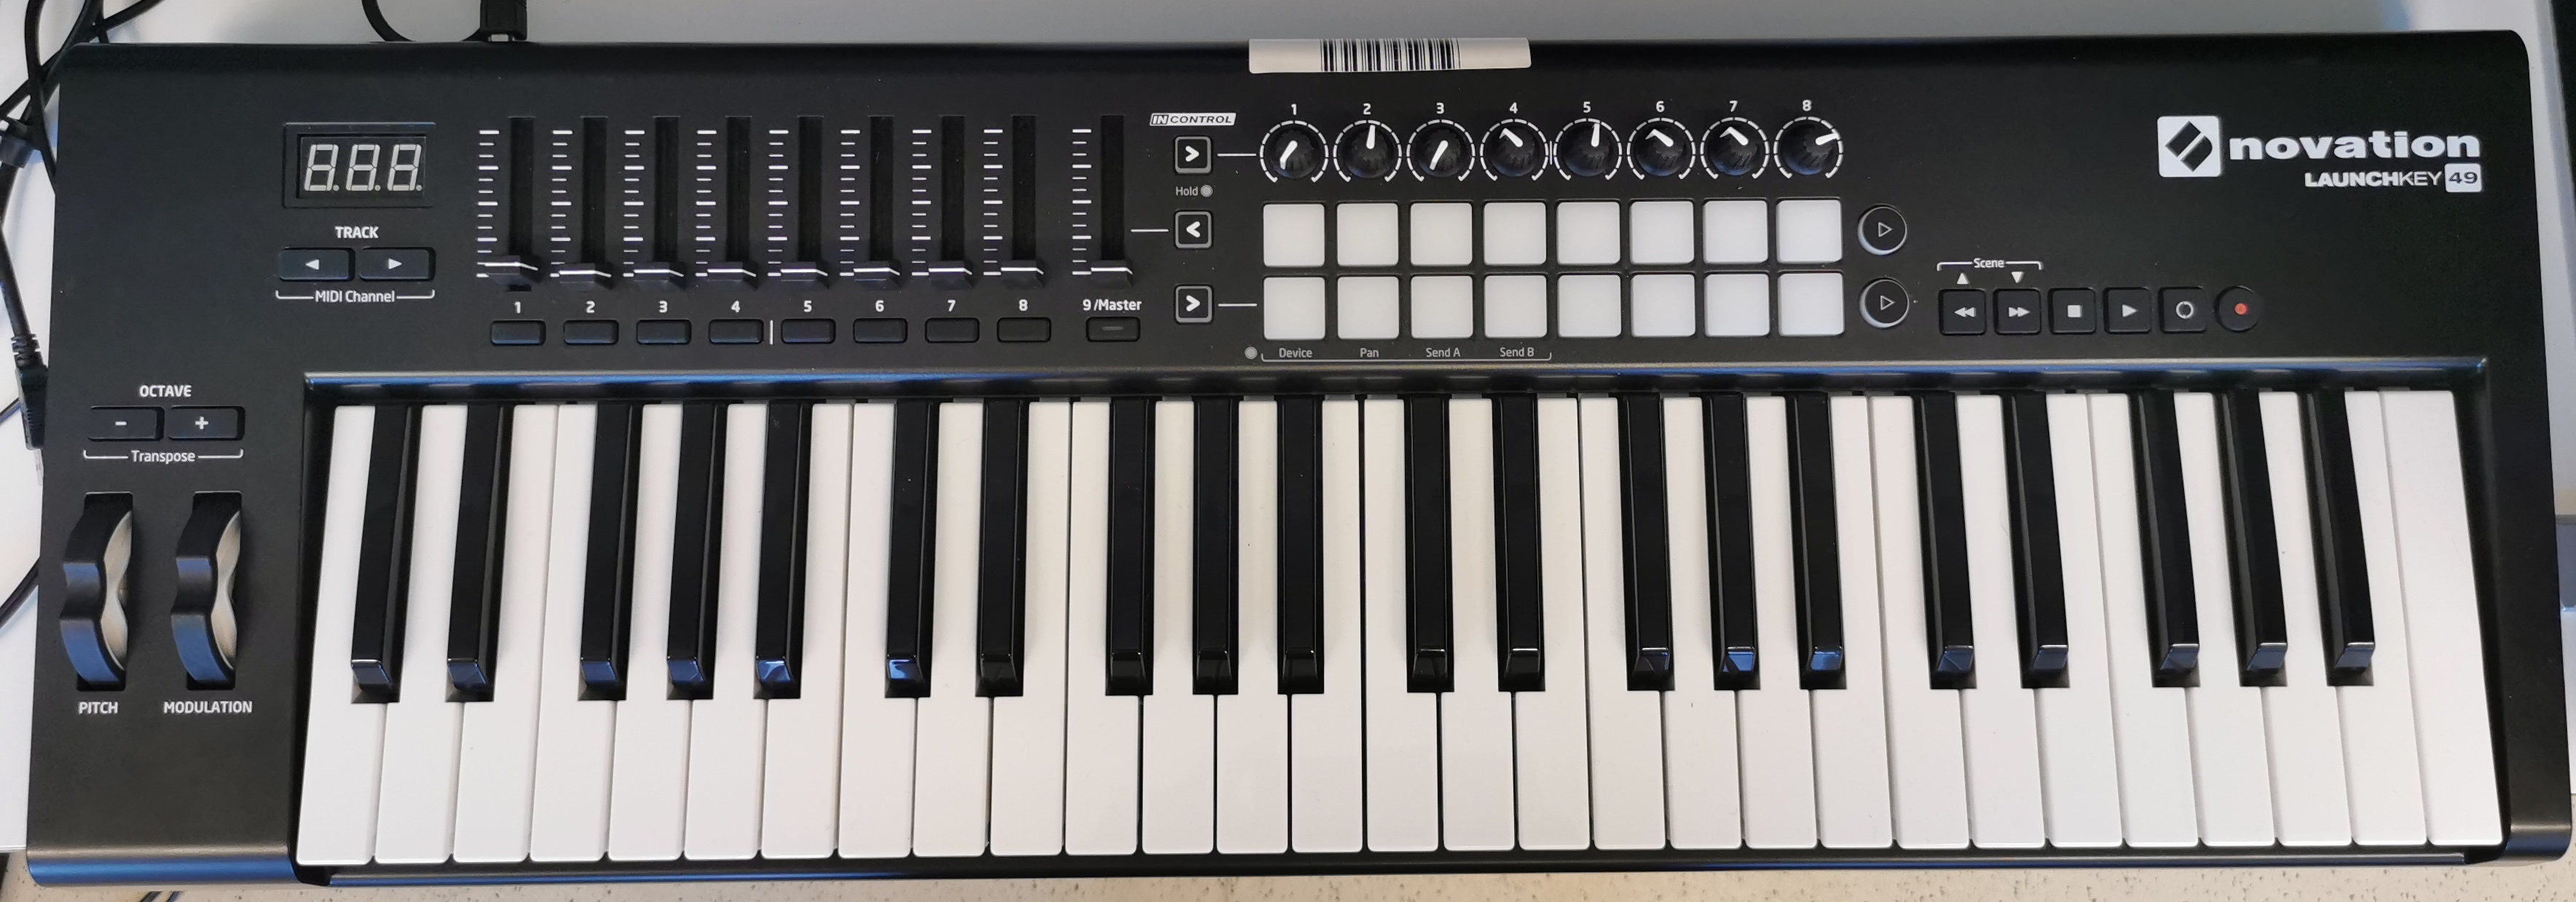
\includegraphics[width=0.7\linewidth]{keyboard}
		\caption{The keyboard being used to control the system}
		\label{fig:keyboard}
	\end{figure}
	
	To play the system, a MIDI keyboard of type Novation Launkey 49 mk2 is used, shown in \ref{fig:keyboard}. For this project, what's been used is the 49 keys that can be played with, 8 knobs, and 9 buttons. The keyboard communicates with unity using MIDI messages, which are read in unity using the MIDIJack package. The MIDI keyboard will be used to enable one to one interactions, with each knob adjusting a specific parameter, and one-to-many interactions with buttons setting all the parameters to specific settings.
	\subsection{System components}
	\subsubsection{Agents}
	The agents have one property to them, which is what position they currently have. This position more specifically represents which pitch they're currently playing at. Each iteration, they will update their position to go towards the pitch with the most other agents, within 7 steps of them in either direction. For the purposes of this system the scale is circular, so if they go beyond the highest pitch they wrap around the the smallest one again. Their movement is limited in that they only have 3 randomly chosen lengths they're able to move, which causes them to spread out a bit more and not move in unison. In addition, if they stay at the same note for a long time, they will be pushed to move towards the pitch nearby that has the lowest amount of agents. How long they stay at the note is determined by a method inspired by the BEECLUST algorithm \cite{schmickl2011beeclust}. The BEECLUST algorithm works by having agents' stop time be determined by how strong a sensor reading is, and here it is instead determined by how many agents are gathered at the position the agent stops at. This behaviour causes the agents to gather up at certain notes for some time, before eventually scattering out and spread between other nearby notes. What's ideal is that this causes some pitches to have agents gather up at them, and therefore rise above the rest, but only for a limited amount of time before it disappears and another pitch has takes over. This is in contrast to the original behaviour of the BEECLUST algorithm, where the agents gather at one point, however here, the ideal point is changing as the agents move, therefore creating a dynamic goal.
	
	\subsubsection{Synthesis}
	The synthesis module takes in all the histograms generated over the system's run, and normalizes them so the highest value in the histogram is 1, while the lowest is 0. Then, each pitch is converted into the corresponding frequency, which is used as the basis for a sine wave. This sine wave's amplitude is afterward determined by how the size of the pitch in the histogram, meaning pitches with few agents can barely be heard, meanwhile pitches with many agents show up more clearly. For each sine wave frequency, the doubled frequency also gets added to the audio output, but at half the amplitude of the original.
	
	\subsubsection{Intermediary System}
	The intermediary System handles the data being transmitted between the agents and the synthesizer works by first simulating the agents for a set number of cycles, and saves the histogram of the agents spread over the pitches for each time step. After the simulation is complete, the saved histograms are sent to the synthesizer and turned into audio output. This means that the system is offline, and can therefore not allow for real time interaction, where a human player can affect the system and how the agents move.
	
	\subsubsection{MIDI keyboard}
	The main way for the user to interact with the system is through the MIDI keyboard shown in figure . This is done in three different ways:
	\begin{samepage}\begin{enumerate}
		\item By playing the keys on the keyboard
		\item By turning knobs on the keyboard to adjust parameters
		\item By pressing buttons to activate certain preset modes of behaviour
	\end{enumerate}\end{samepage}
	The parameter adjustment and modes of behaviour will be discussed separately in the following two sections.
	
	When the user presses the keys on the keyboard, they are able to interact with and influence the swarm. This is done by modifying the array attracting the agents towards certain pitches. The pitches corresponding with the keys the user is pressing down gets extra weight in the attractor array. This causes the agents to be more inclined to go towards those pitches, and so that pitch will get more strength in the output of the audio.
	
	\subsubsection{Visualization}
	The visualization component of the system is rendered in real time in Unity. The state of the system is displayed as one bar for each pitch. The bar to the furthest left is the lowest pitch, and the bar on the right is the highest pitch. The bar gets filled up, with the biggest bar filling up it's entire section of the screen. When the system is generated, each agent is assigned a randomly chosen RGB Hex colour. The colour of the bar in the visualization is the average of the colours of the agents that are currently on that pitch.
	
	\subsection{Parameters}
	These parameters allow the user to interact with the swarm system in real time. They are modified by turning the knobs on the keyboard.
	
	\subsubsection{How long the agent will remain}
	This parameter controls how long the agents will remain at the same note, before it has to move somewhere else. When the agent remains for a long time, it will cause the swarm to gather up at popular notes, causing them to be highlighted. When the agents move away almost immediately, the system is more chaotic. 
	
	\subsubsection{How much impact the MIDI instrument has}
	This parameter controls how much the notes being played on the MIDI keyboard will affect the agents. The higher this parameter is, the more the agents are influenced by the notes being played on the MIDI keyboard compared to the other agents. This causes the agents to cluster around the notes being played on the keyboard.
	
	\subsubsection{Timestep length}
	This parameter controls how long it takes between each update step. This affects the entire system, and determines the tempo of the system. 
	
	\subsubsection{Number of agents}
	This parameter controls how many agents are currently active. This is done by at the start of the system generating the max number of agents, but when updating agents, the loop stops when it reaches the number of agents. In addition, the histograms generated stops adding to themselves when it has added the number of agents. This causes the agents who are not updated to be frozen still until they are reenabled, but they will not influence the system in any way, neither by attracting other agents or audio synthesis.
	
	\subsubsection{Swarm Volume}
	This parameter controls the volume the swarm plays at.
	
	\subsubsection{MIDI Volume}
	This parameter directly translates to the volume of the keys the user are pressing, being directly translated to the output. 
	
	\subsubsection{Agent Range}
	This parameter describes the furthest the agent is able to move. 
	
	\subsubsection{Agent Look Range}
	This parameter controls how far the agent is able to look when it's looking for which direction to move.
	
	\subsection{Modes of Behaviour}
	This section will describe various modes of behaviour exhibited by the system. These will generally correlate with some parameters having specific values, and are therefore also available in the instruments as presets you can set by pressing a corresponding button. The parameters used for each behaviour will be displayed with the following greek letters:
	\begin{samepage}\begin{itemize}
		\item $\alpha$ - How long the agent remains (Range: 0-50)
		\item $\beta$ - How much impact the MIDI instrument has (Range: 0-10)
		\item $\delta$ - Timestep Length (Range: 0-1)
		\item $\phi$ - Number of agents (Range: 3-10000)
		\item $\pi$ - Swarm Volume (Range: 0-10)
		\item $\tau$ - Keyboard Volume (Range: 0-10)
		\item $\lambda$ - Agent Move Range (Range: 0-49)
		\item $\zeta$ - Agent Look Range (Range: 0-49)
	\end{itemize}\end{samepage}
	If a parameter is not mentioned as part of a behaviour, it means it will not affect the behaviour.\\
	The behaviours will be accompanied by a snapshot of the visualization where applicable, and there will also be attached plots showing the movements of all the agents in the system, and showing the individual path of one singular agent. What's important to note is that the plot showing the movement of all the agents, are the average of the plot of all the agents. This means that pitches that have few agents will be faded, while pitches that have many agents will be clear. Unlike the visualization, which is normalized where the pitch with the most agents is always the highest value, here the highest value can only be achieved if all the agents are on the same pitch.
	
	\subsubsection{Regular instrument}
	\begin{samepage}\begin{itemize}
		\item $\pi$: 0
		\item $\tau$: 2
	\end{itemize}\end{samepage}
	In this mode of behaviour swarm volume is set to 0, meanwhile the MIDI volume is set to its max value. This makes the program work as a regular instrument, as what the user plays on the midi instrument, is what will be output. This mode of behaviour exists to work as a benchmark for the rest of the system, so that it can be compared to playing a regular instrument.
	
	
	\subsubsection{Islands}
	\begin{samepage}\begin{itemize}
		\item $\alpha$: 20
		\item $\delta$: 0.1
		\item $\phi$: 2000
		\item $\pi$: 1
		\item $\tau$: 0
		\item $\lambda$: 7
		\item $\zeta$: 12
	\end{itemize}\end{samepage}
	\begin{figure}
		\centering
		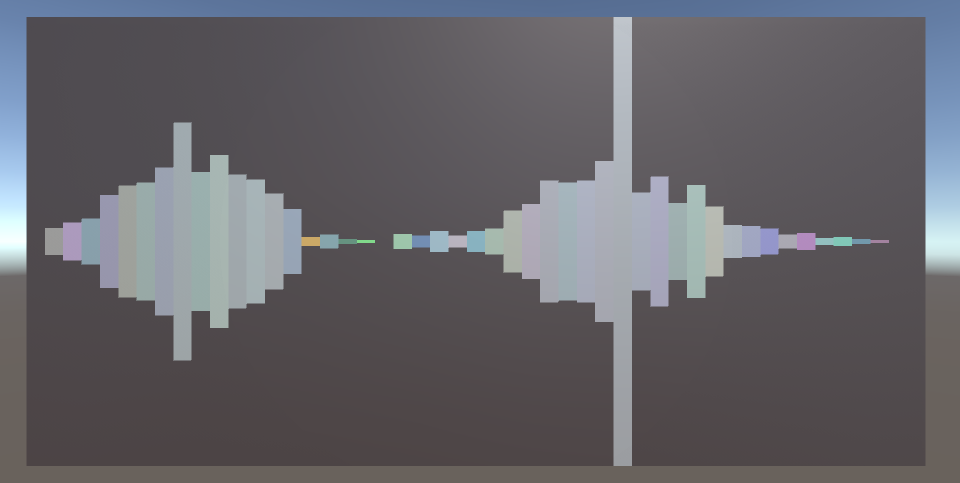
\includegraphics[width=1\linewidth]{islands_vis}
		\caption{The island behaviour}
		\label{fig:islands}
	\end{figure}
	\begin{figure}
		\centering
		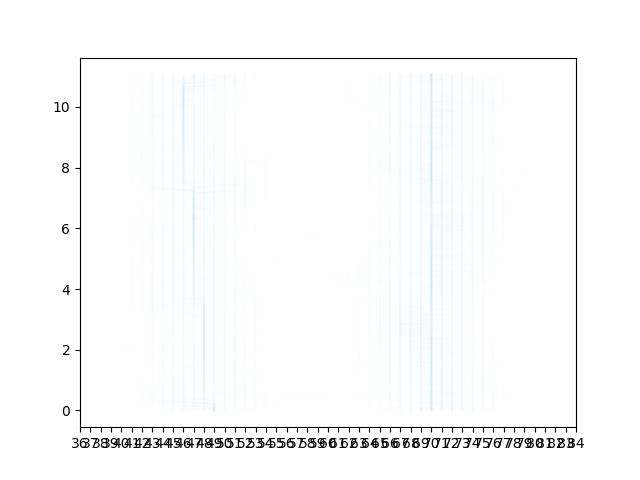
\includegraphics[width=1\linewidth]{islands}
		\caption{The path of all the agents during an instance of the island behaviour}
		\label{fig:islandsAll}
	\end{figure}
	The Island behaviour is characterized by the pitches that have the most agents in their area, having all the pitches next to them have a smaller amount of agents that gradually decrease the further you get from the local optima.
	
	
	\subsubsection{Every other note}
	\begin{samepage}\begin{itemize}
		\item $\alpha$: 30
		\item $\delta$: 0.1
		\item $\phi$: 2000
		\item $\pi$: 1
		\item $\tau$: 0
		\item $\lambda$: 49
		\item $\zeta$: 1
	\end{itemize}\end{samepage}
	\begin{figure}
		\centering
		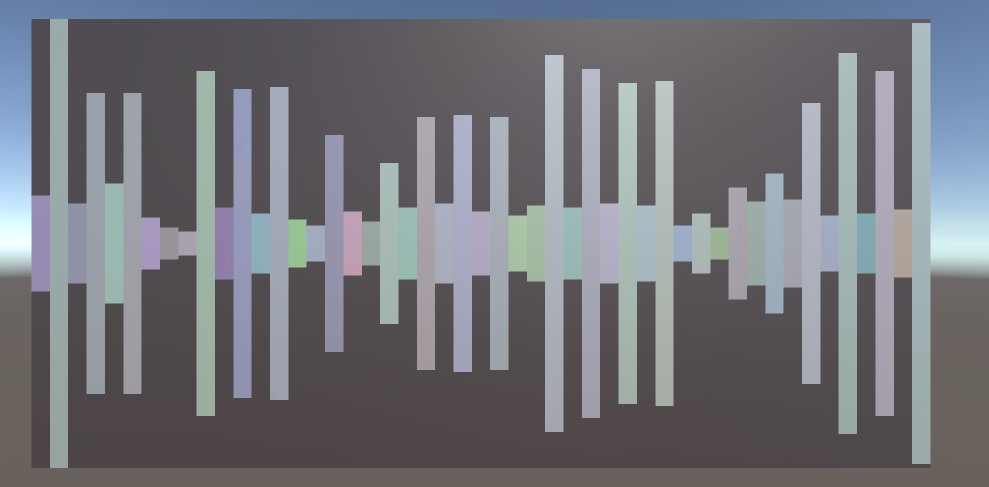
\includegraphics[width=1\linewidth]{even_space}
		\caption{The even spaced behaviour}
		\label{fig:evens}
	\end{figure}
	\begin{figure}
		\centering
		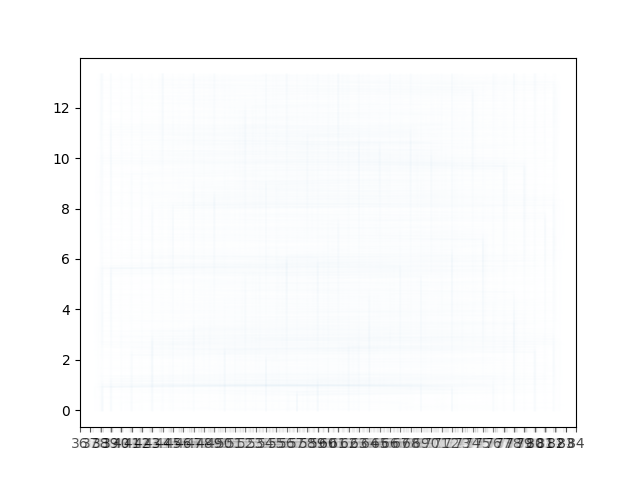
\includegraphics[width=1\linewidth]{even}
		\caption{The path of all the agents during an instance of the even behaviour}
		\label{fig:evenAll}
	\end{figure}
	\begin{figure}
		\centering
		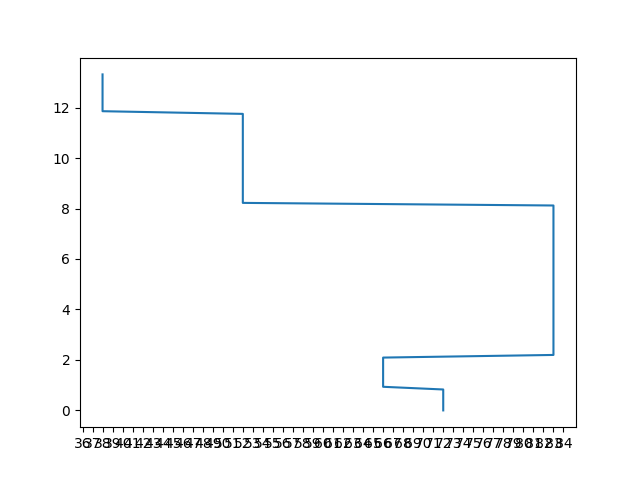
\includegraphics[width=1\linewidth]{evenOneAgent}
		\caption{The path of one agent during an instance of the even behaviour}
		\label{fig:evenOne}
	\end{figure}
	Here, the pitches with most agents are evenly spaced out, with only one or two pitches between them. This causes the audio output to appear somewhat harmonic, as it sounds like all notes belong to a scale.
	
	
	\subsubsection{Few agents}
	\begin{samepage}\begin{itemize}
		\item $\alpha$: Variable
		\item $\delta$: 0.1
		\item $\phi$: 3
		\item $\pi$: 1
		\item $\tau$: 0
		\item $\lambda$: Variable
	\end{itemize}\end{samepage}
	\begin{figure}
		\centering
		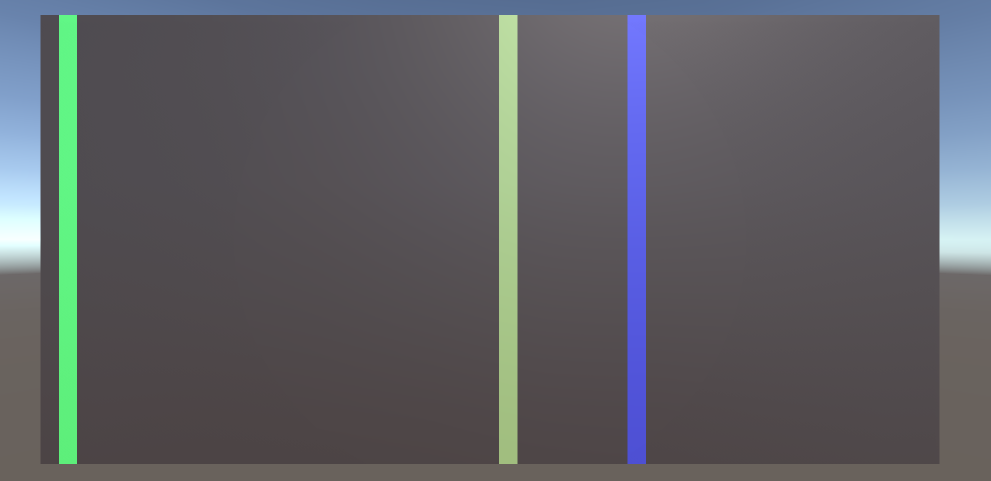
\includegraphics[width=1\linewidth]{few_agents}
		\caption{The few agents behaviour}
		\label{fig:few}
	\end{figure}
	When the number of agents is very low, the output also takes on more of a harmonic approach. This having only a few agents, lead to few notes being played, which will much easier harmonize, due to being distinct pitches that change regularly.
	
	
	\subsubsection{Small movements}
	\begin{samepage}\begin{itemize}
		\item $\alpha$: 0
		\item $\delta$: 0.1
		\item $\phi$: 2000
		\item $\pi$: 1
		\item $\tau$: 0
		\item $\lambda$: 1
		\item $\zeta$: Variable
	\end{itemize}\end{samepage}
	\begin{figure}
		\centering
		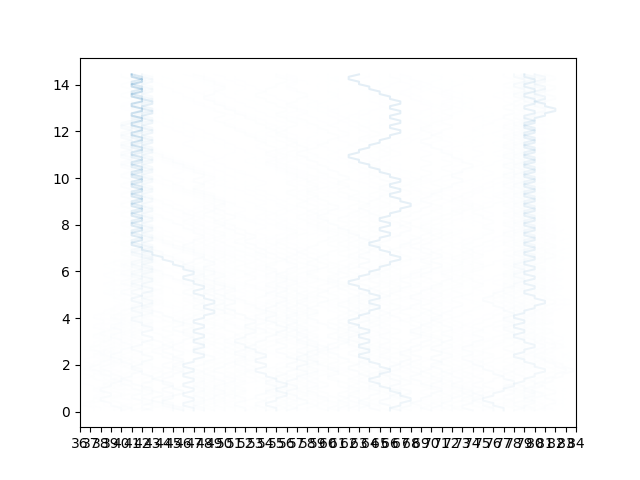
\includegraphics[width=1\linewidth]{smallMovements}
		\caption{The path of all the agents in the small movement behaviour}
		\label{fig:small}
	\end{figure}
	\begin{figure}
		\centering
		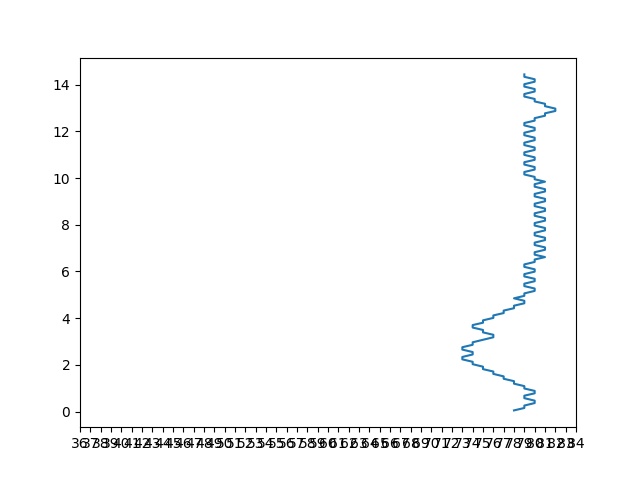
\includegraphics[width=1\linewidth]{smallMovementsOneAgent}
		\caption{The path of a singular agent in the small movement behaviour}
		\label{fig:smallOne}
	\end{figure}
	By restricting agents so that they can only move to one of their neighbours, the system will have very gradual movements, similar to a chromatic scale.
	
	
	\subsubsection{Swarm instrument}
	\begin{samepage}\begin{itemize}
		\item $\alpha$: 25
		\item $\beta$: 10
		\item $\delta$: 0
		\item $\phi$: 10000
		\item $\pi$: 1
		\item $\tau$: 0
		\item $\lambda$: 7
		\item $\zeta$: 49
	\end{itemize}\end{samepage}
	\begin{figure}
		\centering
		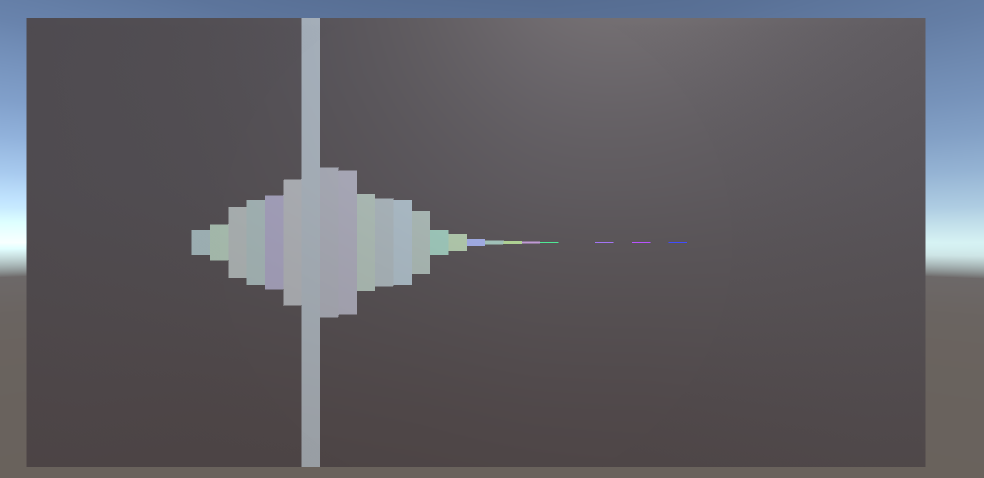
\includegraphics[width=1\linewidth]{instrument}
		\caption{The instrument behaviour when holding down one note}
		\label{fig:swarminst}
	\end{figure}
	\begin{figure}
		\centering
		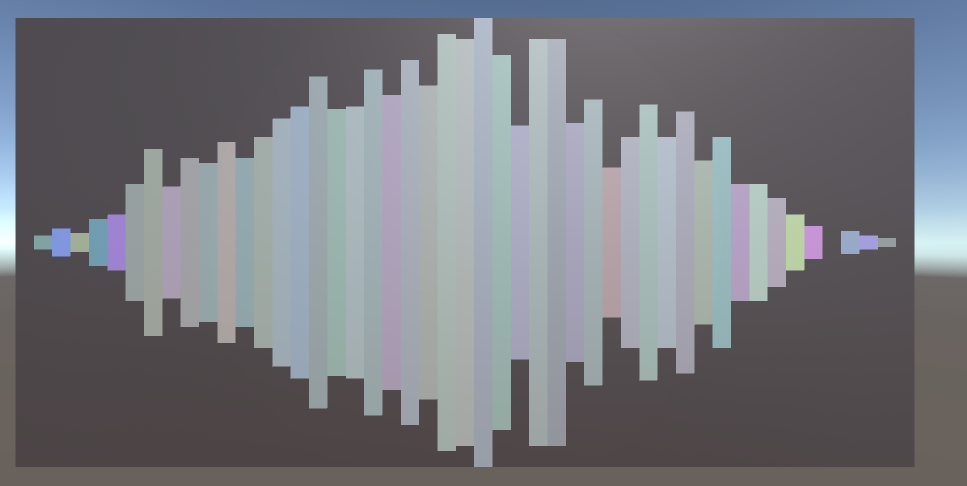
\includegraphics[width=1\linewidth]{instrument_move}
		\caption{The instrument behaviour moving from one note to another}
		\label{fig:swarmmove}
	\end{figure}
	
	This is another simulation of an instrument, but this time it is done purely by changing the parameters of the swarm. This has the side effect that you're only really able to play one note at a time, as if you play more the agents will converge on one of the notes being played. This behaviour also has the side effect of that since the agents themselves have to move from one note to another, if you implement a big leap between the notes played, the agents will travel to the desired pitch over time, simulating the effect of dragging your fingers across a piano.\\
	This behaviour was designed as an alternative benchmark to the regular instrument behaviour, as it didn't implement the swarm system at all. It was desirable to have a benchmark that was created by adjusting the parameters of the system as well, as that would give a set of parameters that were determined to be as close to a regular instrument as possible.\\
	\begin{figure}
		\centering
		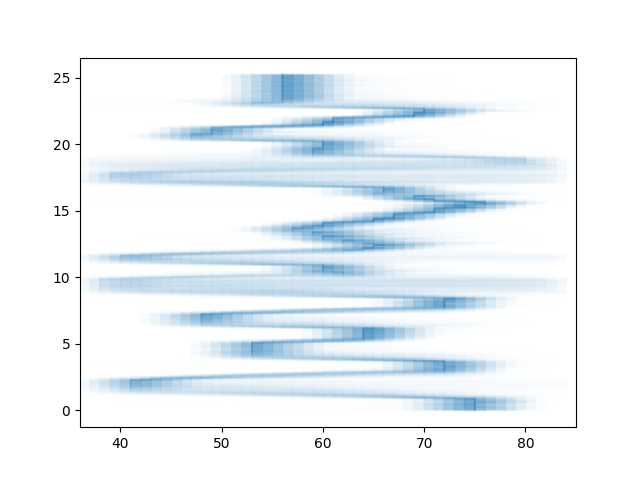
\includegraphics[width=1\linewidth]{swarminstrument}
		\caption{The path of all the agents during an instance of playing the swarm instrument}
		\label{fig:swarm}
	\end{figure}
	\begin{figure}
		\centering
		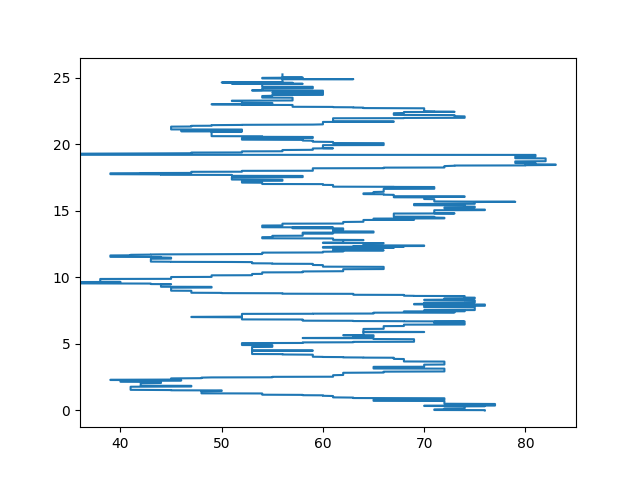
\includegraphics[width=1\linewidth]{swarminstrumentOneAgent}
		\caption{The path of one agent during an instance of playing the swarm instrument}
		\label{fig:swarmOne}
	\end{figure}
	\ref{fig:swarm} shows the movement of all the agents during an instance of playing the swarm instrument. Compared to previous graphs of all agents, this graph looks much more blurry. The answer to why this is can be seen when \ref{fig:swarmOne}, which shows the path of only one agent in the same simulation, is compared with \ref{fig:swarm}. The single agents moves back and forth around the pitch that is most highlighted in the graph of all the agents, and this causes a blurriness. The reason the agents are going back and forth around the central pitch so much is because the system update time is set to it's minimum, causing the system to update as fast as it possibly can, which in turn causes the agents to be forced to move much more quickly.
	
	
	\subsubsection{All chaos}
	\begin{samepage}\begin{itemize}
		\item $\alpha$: 0
		\item $\delta$: 0
		\item $\phi$: 10000
		\item $\pi$: 2
		\item $\tau$: 0
		\item $\lambda$: 49
		\item $\zeta$: 49
	\end{itemize}\end{samepage}
	\begin{figure}
		\centering
		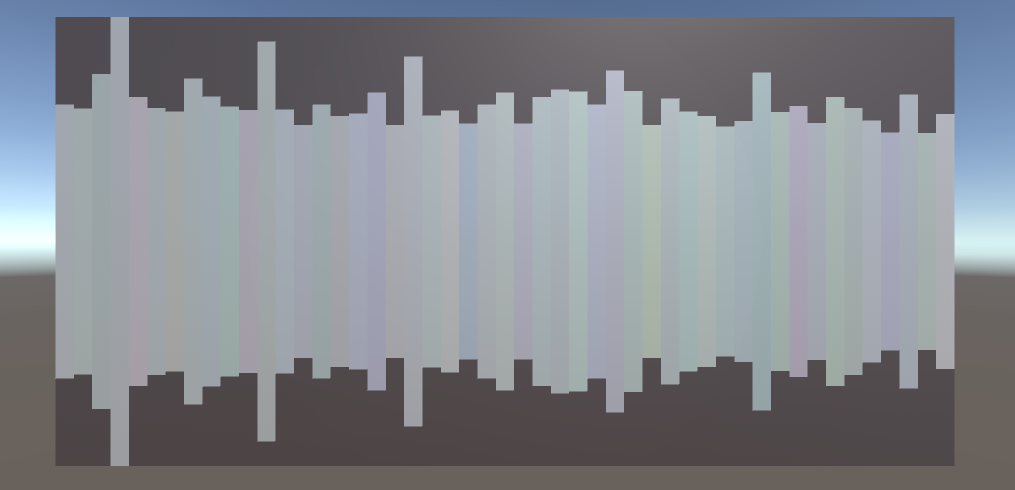
\includegraphics[width=1\linewidth]{chaos_vis}
		\caption{The chaotic behaviour}
		\label{fig:chaos_vis}
	\end{figure}

	In this mode, the agents are able to jump to any note when they move, causing them to jump around randomly. In addition, agents are not allowed to stay on the same pitch, meaning that they're always jumping from one note to the next, and the time is set to the minimum, causing them to move around as fast possible.
	\begin{figure}
		\centering
		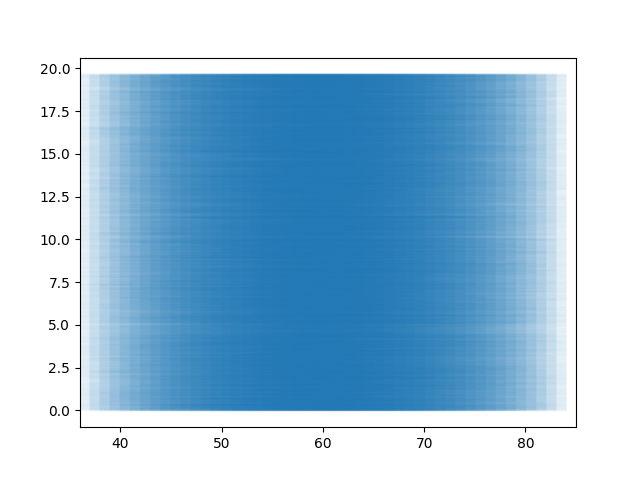
\includegraphics[width=1\linewidth]{chaos}
		\caption{The path of all the agents during an instance of the chaotic behaviour}
		\label{fig:chaos}
	\end{figure}
	\begin{figure}
		\centering
		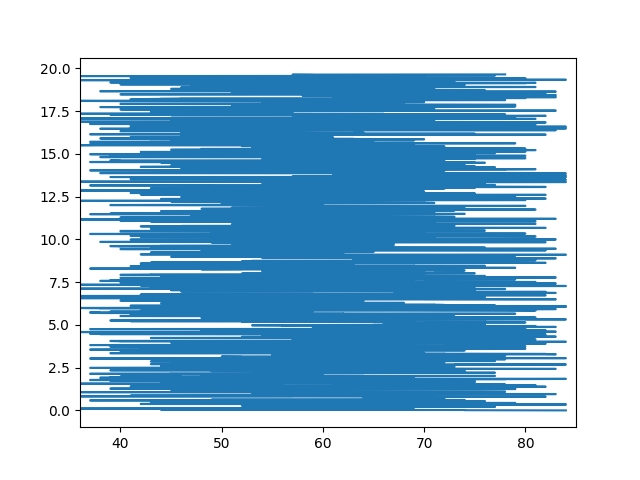
\includegraphics[width=1\linewidth]{chaosOneAgent}
		\caption{The path of one agent during an instance of the chaotic behaviour}
		\label{fig:chaosOne}
	\end{figure}
	\ref{fig:chaos} shows the movement of all the agents, and 
	
	\subsubsection{Zooms around}
	\begin{samepage}\begin{itemize}
		\item $\alpha$: 0
		\item $\delta$: 0
		\item $\phi$: 10000
		\item $\pi$: 2
		\item $\tau$: 0
		\item $\lambda$: 1
		\item $\zeta$: 1
	\end{itemize}\end{samepage}
	\begin{figure}
		\centering
		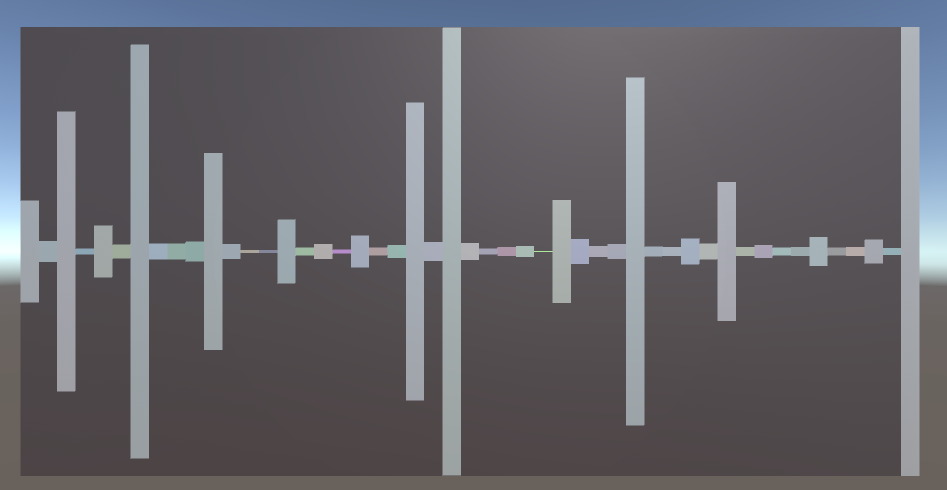
\includegraphics[width=1\linewidth]{zoom_vis}
		\caption{A still shot of the behaviour where the agents move around very fast}
		\label{fig:zoom_vis}
	\end{figure}
	\begin{figure}
		\centering
		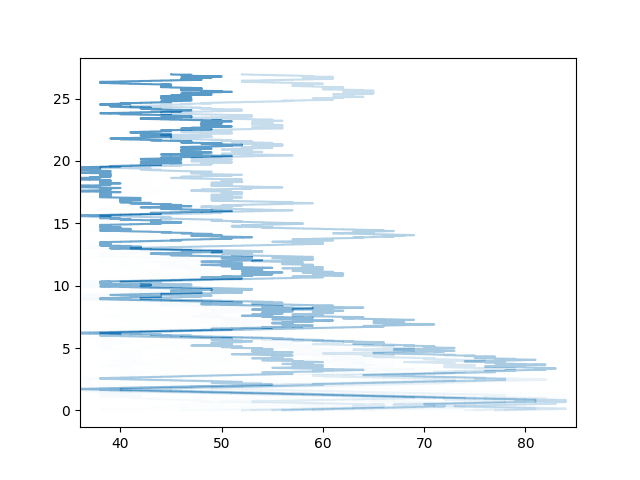
\includegraphics[width=1\linewidth]{zoom}
		\caption{The travelled path of all the agents in the system with the zoom behaviour}
		\label{fig:zoom}
	\end{figure}
	\begin{figure}
		\centering
		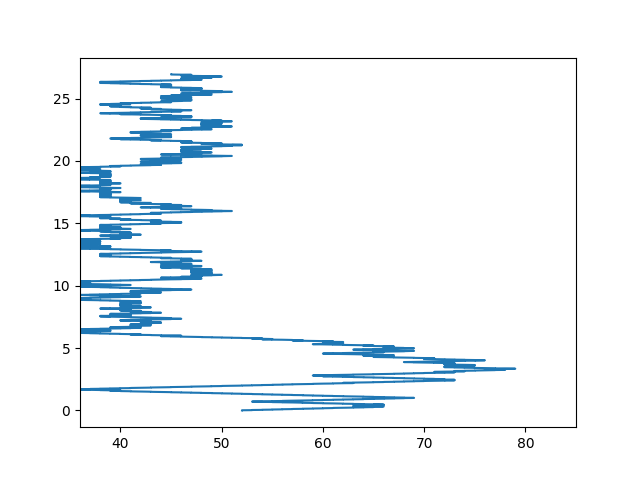
\includegraphics[width=1\linewidth]{zoomOneAgent}
		\caption{The travelledpath of one individual agent in the system with the zoom behaviour}
		\label{fig:zoomOne}
	\end{figure}
	This mode has similar parameters to the previous one, but instead of the range of the agents movements being the max range, it is instead just able to move to its neighbours, and the same goes for how far it is able to see when it determines which pitch to move towards. This behaviour is characterized by the agents moving around very quickly, with most of the agents gathered at one pitch.
	
	\chapter{Evaluation}
	To answer the research question of `How do people interact with a swarm-based music system?', we want to conduct a thematic analysis of users who interact with the system. To perform a thematic analysis, a data set is needed of people's experience interacting with the system, and for this purpose we have conducted a user study. As mentioned in the background, a thematic analysis requires some questions to be answered beforehand, which will be answered here. \\
	Firstly, on the question of what counts as a theme we will count anything that multiple participants in the study mentioned, that relates to the question of how they interact with the system. Due to this, we will focus on the dataset as a whole, instead of looking at any one specific aspect of the interaction. Our approach to finding themes will be done both deductively and inductively, with some things being specifically asked for in the user study, but there will also be themes found inductively, as we don't know how people will describe their experience with the system beforehand. The analysis of the data itself will mostly be on a semantic level, mainly focusing on the participants' reported experience with the system, but there will also be some latent analysis, trying to understand why the participants had the experience they had.
	\section{User Study}
	The user study consisted of the participants doing various task while manipulating the knobs, saying how they responded to various behaviours, and a section where they could play freely with the instrument. All of the tasks were done twice, once when the participant could not see the screen, and one where they could, to see if the impression of the system changed depending on the visual feedback. The study involved 8 participants with varying levels of experience, from participants who only listened to music, through participants playing music at a hobby level, to participants creating music and instruments in their free time. Before the task all the participants got a quick demonstration of the different parameters, so they have an idea what each parameter did. In addition, the knobs are labelled with what parameter it changes.
	
	\subsection{Adjust parameters to create sounds}
	In the first section of the user study, the participant was asked to create a certain type of sound. The sounds they were tasked to create were:
	\begin{samepage}\begin{enumerate}
		\item A chaotic sound
		\item A pleasant sound
		\item A sound they could control
		\item A sound they could not control
		\item A duet with the system
	\end{enumerate}\end{samepage}
	The participants where given free reign to adjust the parameters as they wanted to, with some exceptions for the tasks regarding controllable and uncontrollable sound, where certain parameters were restricted to as they would invalidate the task.\\
	The reason for asking these questions are twofold. The main motivation is to make sure the participants get familiar with the system, by experimenting with changing the parameters. The second reason is that
	\subsubsection{Chaotic sound}
	\begin{displayquote}
		I think chaos is pretty easy to accomplish here.
	\end{displayquote}
	The first task consisted of making a sound that is as chaotic as possible. While chaotic can mean different thing, it is left up to the participants to decide what kind of sound they want.\\
	When the participants tried to create a chaotic sound without seeing the screen, they tended to find it quite easy and were easily satisfied. When looking at the visual feedback however, the participants talk about how it changed their opinion on what a chaotic sound was, as the feedback informed their opinion of that.
	\subsubsection{Pleasant sound}
	\begin{displayquote}
		There is a specific sound I have in my head that I think the system could make, but I didn't get quite there.
	\end{displayquote}
	Similar to the previous task, the participants were asked to make a sound they found pleasant, with them deciding what kind of sound they want themselves. When not seeing the screen, most participants found themselves struggling, finding it hard to influence the system in the way that they want. When seeing the screen opinion was much more split, as some participants found it much easier to influence the system when they got the visual feedback of how the system responded to their parameter changes, while others still found it quite hard, and mainly thought it was due to lack of experience.
	\subsubsection{Controllable sound}
	\begin{displayquote}
		I feel like I can affect it, but not control it.
	\end{displayquote}
	This task's goal was for the participant to make a sound they felt they were able to control by playing the keyboard. For this task, the keyboard volume had to be at 0, so that the participant could not simply manipulate the sound directly by playing the keyboard. Participants generally found this task to be very challenging, especially when not seeing the screen. Some participants thought it was easier when they were able to see the screen, but many were still struggling and found it unintuitive.
	\subsubsection{Uncontrollable sound}
	\begin{displayquote}
		I'm not affecting anything and I can tell!
	\end{displayquote}
	The next task was the opposite, to make a sound they couldn't control with the keyboard. The limitation here is that they could not set keyboard impact to 0, as that again would invalidate the task. Participants all found this task to be very easy, especially not when seeing the screen. When seeing the screen, some participants found the task to be a bit harder, as they were much more able to see the small changes the keyboard caused, but it was still considered quite simple. Most participants solved this task either by increasing the move range to it's maximum, so the agents would randomly jump everywhere, or setting it to a minimum, so that they can't move at all. In addition, some participants solved it by increasing the timestep update to be every second, which causes the system to run very slowly, and taking a very long time to adapt to the input from the keyboard.
	\subsubsection{Duet}
	\begin{displayquote}
		Feel like I'm making random sounds, but also that the swarm is helping me a bit.
	\end{displayquote}
	The last task was to try and play a duet with the system. The participants generally found this hard to do without seeing the screen, stating that the system feels uncooperative, and that it's hard to play with the random notes that it plays. When seeing the screen, participants found the task to be easier, but still feel a bit hampered by the system playing randomly, and not cooperating to play in the same key as the participant.
	
	\subsection{Parameter Evaluation}
	After completing the tasks, the participants were asked how they feel about the various parameters, and how it felt to adjust them and how intuitive they were.
	\subsubsection{How long the agent will remain}
	\begin{displayquote}
		It's nice, has a clear effect.
	\end{displayquote}
	The participants generally liked using this parameter, and said that it helps them controlling the sound and it is fun to see and hear the effects of using it.
	\subsubsection{How much impact the MIDI instrument has}
	\begin{displayquote}
		Didn't play much with it, tended to be either at the minimum or the maximum.
	\end{displayquote}
	The second parameter was less used by the participants, with them either having it on max and not adjusting it, or sometimes setting it to a minimum. Some participants however said they liked using it to determine how strictly they controlled the system, which was important to bring out their ideas.
	\subsubsection{Timestep length}
	\begin{displayquote}
		I mix it up with the note length one, but otherwise pretty intuitive.
	\end{displayquote}
	The timestep length parameter was generally liked by the participants, though some found it a bit unintuitive. Multiple participants said they mixed it up with note length, and that they felt they fulfilled a similar purpose in the system. One user also stated that they felt it was the most important parameter to determine whether or not they had control.
	\subsubsection{Number of Agents}
	\begin{displayquote}
		Liked it a lot, it's cool that you can add and subtract, and you can immediately hear the difference.
	\end{displayquote}
	The participants liked modifying the number of agents, and felt that it created different and interesting sounds depending on how many agents were present. Some considered many agents to be more chaotic, and low agents made it more controllable. Another participant described it as many agents causing lots of sounds while few agents sounded like castle music from old Mario games.
	\subsubsection{Swarm Volume}
	\begin{displayquote}
		I used it to mix the noise with the keyboard.
	\end{displayquote}
	For this parameter, the participants were generally divided into two camps. Either, they didn't change it much at all, keeping it in it's default position. Some participants also noted that they tried to keep the system noise down, as the loudness scared them.

	\subsubsection{MIDI Volume}
	\begin{displayquote}
		It's fun to hear how you stand out in comparison to the other agents.
	\end{displayquote}
	The general opinion of the participant is that this parameter is intuitive, and easy to understand what use it has. One talked about how they preferred using that knob to influence the balance between swarm and keyboard, as opposed to using the swarm volume parameter to influence that.
	\subsubsection{Agent Range}
	\begin{displayquote}
		Use it very closely together with look range, to define the moves of the agent.
	\end{displayquote}
	The participants had a generally positive opinion of adjusting this parameter, liking both how it plays a chromatic scale at low settings, and how it creates a more chaotic setting when it is higher. Some users however also found it a bit confusing, and that it took some getting used to, as adjusting the parameters didn't always create the sound they were going for. Many participants also mentioned how they felt the parameter was very closely linked to the agent look range.
	\subsubsection{Agent Look Range}
	\begin{displayquote}
		Very closely connected to the move range.
	\end{displayquote}
	Most participants thought that the look range and move range were very interchangeable, and was confused about the difference between the two parameters. Therefore most participant either kept it very high or very low. Some participants however, found this parameter to be more understandable than the move range instead.
	\subsection{Behaviour Evaluation}
	Next, the participants were shown the presets one after another, and asked to give their thoughts on them. The participants were shown each preset twice, first without seeing the screen and then once more right afterwards where they could see the screen.
	\subsubsection{Regular instrument}
	\begin{displayquote}
		It's just a piano.
	\end{displayquote}
	Participants generally found this behaviour to just be like a piano. When they saw the visual feedback, they found that it was very unresponsive.
	\subsubsection{Islands}
	\begin{displayquote}
		I like the sound, has this undulating thing going on. A lot of texture and different things happen. I don't feel I have control.
	\end{displayquote}
	The second preset were described by the participants as scary, organ-like, and like a keyboard that doesn't want to cooperate. With the visual feedback, the participants felt they were more in control, as they could see the small movements in the system, even if they weren't able to hear them.
	\subsubsection{Every other note}
	\begin{displayquote}
		This one is much more slowly evolving, which I like about it.
	\end{displayquote}
	The participants generally felt that this behaviour was slow and dramatic. Some said that it sounded like the music that would play when a bad guy enters in a horror movie, while another said it sounded like the church organist had gotten a drinking problem. The impressions didn't change much when they saw the visual feedback, though some noted that it looked different from what they expected.
	\subsubsection{Few agents}
	\begin{displayquote}
		Mario castle!
	\end{displayquote}
	This behaviour was mostly considered pleasant by the participants. Many of the participant also described it as calming, while some felt it was a bit unsettling. Some of the participants thought they had control over the system when they played without seeing the screen, but when they saw the screen they realized that they had no control.
	\subsubsection{Small movements}
	\begin{displayquote}
		This is nice, reminds me of one of those crazy chromatic Chopin tunes.
	\end{displayquote}
	The participants generally described this behaviour as very exciting and energetic, and comparisons were made to chase scenes from 80's science fiction. When seeing the screen, one of the participants noted that the movements of the agents also looks like a chase scene, and another said they liked how the pitches end up converging.
	\subsubsection{Swarm instrument}
	\begin{displayquote}
		Extremely responsive. I feel like if I could play the piano this would be fun. This has some interesting sounds.
	\end{displayquote}
	The behaviour was described as very responsive and controllable. It was also described as an organ with glissando, or alternatively as if you drag your hand over a piano. Some participants noted that it sounded a bit like a broken keyboard, that took some time to get to where you wanted it, but that that was a benefit. When seeing the screen the participants said that it corresponded well to what they expected, but that it was pretty to look at. However one participant noted that the behaviour wasn't very good for moving between notes that are close to each other.
	\subsubsection{All chaos}
	\begin{displayquote}
		Scorched earth thing. Sounds like Smashing Pumpkins, heavy sound, distorted electric guitar.
	\end{displayquote}
	The participants described this behaviour as very chaotic and it being completely uncontrollable. In addition, some participants talked about how it sounds like something really disturbing is happening in a horror movie. The visuals really didn't affect or change any opinions of the behaviour.
	\subsubsection{Zooms around}
	\begin{displayquote}
		A rollercoaster of sounds.
	\end{displayquote}
	This behaviour was described as insect-like by the participants, with comparisons being made to bees and ants, coming towards the participant and flying or scurrying around. It was also described as unstable, and compared to the sounds of tuning a radio. The visual feedback for the behaviour was received well, and it was described as fun and fascinating to look at, with one participant mentioning that it looks like a weird 80's video game.
	\subsection{Freeplay}
	As the final part of the user study, the participants were given free reign to play whatever they want on the system, including switching between parameter control and the presets as they wish.
	\subsubsection{Preference of parameters vs behaviours}
	\begin{displayquote}
		Preferred the knobs, the presets are fun but I prefer to alter them myself.
	\end{displayquote}
	Between the participants, the vast majority preferred tuning the parameters themselves, and did not even touch the preset behaviours. The stated reasons for this preference is that the presets didn't really do what the participant wanted, or that it's more fun and engaging to alter the parameters themselves. There was however two participants who preferred the presets, one citing that it felt easier and much less messy to use the presets, and the other one specifically mentioning the swarm instrument behaviour as very fun to play with.
	\subsubsection{Overall impression of the system}
	\begin{displayquote}
		There's a lot going on with this system. Could probably spend a lot of time exploring it.
	\end{displayquote}
	The participants' overall impression of the system was positive, with many saying that they enjoyed using the system. Multiple participants mentioned how it was fun to see how the agents reacted to the keyboard, and how they moved around in response. Some participants mentioned that they felt they were not skilled enough with music to bring out the full potential of the system, and wished they had had that experience so they were able to use it more competently. Participants also talked about how they struggled to control the system at first, but how they over time got more comfortable with it and started to understand the system. One participant in particular mentioned how they looked a lot at the visual feedback at the start, but over time grew less dependent on it and started listening more, almost feeling that the visual feedback was a distraction. Other participants however, felt that the screen was a huge help, and that they were more in tune when they could see how the agents are spread out.
	\section{Thematic Analysis}
	\iffalse
	From the data gathered during the user study, four main themes were discovered. These themes are:
	\begin{samepage}\begin{enumerate}
		\item Preference of parameters or behaviours
		\item The effect of the visualization
		\item Is the system an instrument or a musical partner? 
		\item How is the sound perceived?
	\end{enumerate}\end{samepage}
	\subsection{Parameters vs. Behaviours}
	One of the themes that were directly asked for in the user study was whether the participant preferred to use the knobs to tune the parameters or buttons work with the presets. Most participants said that they preferred the knobs, and in fact, they didn't even use the presets. The participants said that they really liked the control they get over the system when they are modifying the knobs, and that it's engaging to see how the system changes. This highlights how the ideal for interacting with the system is that it's an experience where the participant takes an active part in creating the musical space. This can also be seen in the participants who preferred the presets, as the favored preset among them was the swarm instrument where they're able to direct the swarm directly. This is also reflected in how the participants felt about the different presets, with the swarm instrument being the most popular preset.\\
	Another thing to note is that the two participants who preferred using the presets, were also the participants with the least musical experience of everyone interviewed, and were the only participants who didn't play an instrument. This could be due to the premade behaviours being easier to interact with when you have less experience creating music, as they will easier make interesting sounds. Meanwhile, more experienced musicians with familiarity about how to create the sounds they want, rather wanted to experiment with the whole musical space, which can only be accessed by adjusting the parameters yourself.\\
	This leads back to a question of how much control is desired in the system. This is especially interesting as compared to conventional instruments, the pitch swarm agents give the user much less control over the audio output. 
	\subsection{Visualization}
	Visualization was the other theme we specifically asked for in the user study, as we asked the participants how they felt doing the tasks both with and without the visualization. This was asked for, because seeing how people interact when they have just the sound to guide them and how they interact when they can see the exact state of the system. 
	\subsection{Instrument vs. Musical partner}
	Another interesting theme is how the participants approached the system, and whether they saw it as an instrument or a musical partner. When the participants were recruited to the user study, the system was described as an instrument based on how bees move, and this may have biased the participants to think about the system as an instrument. From the duet task, many of the participants said they felt like the system wasn't trying to play with them, and therefore felt they struggled with the task. Other participants talked about how they felt the system helped guide them to certain ideas they hadn't considered themselves. These two opinions highlight the difference between seeing the system as an instrument to be played, and a musical partner to cooperate with. 
	\subsection{How the sound is perceived}
	Many participants mentioned how they felt the sound sounded like something from the 80s, specifically either sci-fi shows or video games, with mentions of Doctor Who and Mario.	
	
	\fi
	\subsection{Control}
	An interesting aspect of the system is the level of control the user has. In regular instruments, like a piano or a guitar, the user has very precise control of which sound is outputted, but this is not the case with the pitch swarm agents. Due to the agents acting on their own regardless if they get input from the keyboard or not, there is always a degree of randomness to the created sound that is not present in conventional instruments. This challenges the perception that the system is an instrument at all, and could be seen closer to a musical partner you're playing with, like for example a bandmate. However there is still a central difference here, as with a bandmate there is usually some kind of coordination agreed upon beforehand, or at the very least, a common understanding of the musical language from consuming music. With the pitch swarm system, that common understanding is not present, as the basis for choosing which pitch the agents move to is decided only by where the other agents are.\\
	This dilemma showed up in the task where the participants were to play a duet with the system. Some participants felt that they failed at it, because the system was following no rhyme or reason when they were playing. Other participants however, felt that they were able to play a little duet, and that the system followed them adequately. The main difference in the approaches by these two groups is that one group often had a clear idea in mind of what they wanted to hear, and was trying to force the system to play that idea. The other group however, was more willing to be led by the system to ideas they hadn't considered. This shows a difference in the desired level of control between the participants, with the first group generally wanting more precise control over the audio they create while the second group are more willing to go with the flow of what it creates.\\
	This is also relevant to the question of preferring tuning the parameters yourself or using the preset behaviours. The presets are much better at giving a specific type of sound, but the trade-off is that you're stuck with that sound. On the other hand, tuning the parameters directly allows you the change the output sound, but it's also a bigger musical space you have to search through. In the user study, the two users who used the presets, were the two participants with the least musical experience. When asked why they chose them, they said that they felt tuning the parameters directly was more messy, which reflects that there are more musical possibilities when tuning directly, but that a lot of them are not desired. The fact that the participants with less musical experience preferred the presets could also be a reflection of how people with musical experience are more used to exploring the musical space that is available to them. This is reinforced by the statements of the participants who preferred tuning the parameters directly, as they said they liked how exploratory it was, and how it had so many possibilities for them, depending on the configuration they set up.\\
	It is also worth noting that among the presets, the one that was the most popular with the participants was the swarm instrument preset, which is the preset that has the most interaction. In all the other presets, with exception of the regular instrument, there is little control over how the audio sounds. The fact that this preset was so well liked shows how valuable interaction and being able to directly change the output is important for users of the system. The other behaviours, while they can have fun sounds or look interesting in the visualization, are not engaging to interact with in the long run because they are static.\\
	Another aspect of the system regarding the separation of instrument and musical partner is how you feel playing with the system. As the system is a swarm system, consisting of up to 10,000 agents, is this reflected when playing with the system? In the interviews for the user study, there is a trend that the fewer agents that are being played with, the more individual they feel. On the contrary, when there are many agents in the system, the system is rather regarded as a singular entity. The cause for this could be that when there's very few agents, more of them will be playing at the max volume of the system, which makes each distinctive agent clear. On the other hand, when there are many agents, their individual notes blur together to become this collective sound, which is closer to being an average of all their voices. This is also partially due to the fact that the pitch with the most agents will always be played at the max volume, regardless of how many agents are on the pitch.
	
	\subsection{Visualization}
	One thing that was specifically asked for in the user study was how the participants felt that the visualization impacted their experience. The motivation for asking this was that the visualization is a unique element to the system that is not found in most other instruments. The visualization allows the user to get a very precise idea of the audio itself is constructed, showing the exact position of the agents. Because of this, we wanted to investigate how people interacted with the system when they could only use their ears to guide the music, versus how they did when they could also see the visualization, and if that changed the way they played.\\
	Most users felt that their experience changed when they were able to see the visualization for the tasks. Specifically, they felt that the visualization helped them get control of the system, and made it easier to influence the it in a way that they wanted. The act of seeing the visualization also made them aware of their influence even when they couldn't hear anything, as can be seen with the island behaviour. When they tried playing with the island behaviour without seeing the screen, the general opinion of the participants was they they were not able to affect anything by playing. When they were able to see the visualization however, they felt that they had more influence, and could see when agents were attracted to the note they were playing on the keyboard, even when they couldn't hear it. \\
	However, some participants also felt the visualization was not much help, and that rather than help, it got in the way when they got to grips with the system. This could be due to the visualization being distracting, and that it gives something else that has to be considered.\\
	Another aspect of the visualization that was mentioned was that it was fun to look at. This was separate from the increased control the participants felt they had when they looked at the visualization, as they remarked about it being engaging to watch even when the behaviours didn't allow for much control by the user. The participants created stories for the bars that moved around in the visualization, for example describing the small movement behaviour as looking like a chase scene. This is interesting, as the same participant described the sound as sounding like something from a chase scene in a sci-fi movie, and they were therefore connecting the visuals to the association they already had from the audio. It was also suggested that the visualization could be used as something to show the crowds while a performer was using the system. Similar to how the participants felt it was engaging to look at how the system behaved and acted, the visualization could also enhance the concert experience by providing a visual component as well as an auditory one.
	
	
	\chapter{Future Work}
	
	It is over. I solved it. 
	
	\chapter{Conclusion}
	Every major artist alive today should use this. Give money please. Am hungry.
	\bibliographystyle{ieeetr} 
	\bibliography{bibliography} % Entries are in the "refs.bib" file
\end{document}

